%% FullCourse_10Lecs -- Lecture 7, Act 2 (REPRESENT, part 2/2): Word Embeddings
%% ch14 rebuild (2026-07-07), per Lec07_ch14_Rebuild_Plan_2026-07-07.md.
%% Reused frames copied verbatim (with renumbered cross-references) from
%%   archive_pre_split/pre_ch14_rebuild_2026-07-07/Lec07_T1b_Word_Embeddings.tex
%%   (TF/IDF/TF-IDF trio relocated OUT to T2a; one-line recall kept here)
%% New frames follow chapter14 sec. 14.3.2-3: representation-comparison table,
%% hawk-dove direction + separability, time-series pitfalls, corpus/China parallel.

%% Shared preamble for the FullCourse_10Lecs topic decks.
%%
%% Each topic .tex \input's this file, then defines its own \title, \date
%% override (if any), \graphicspath, and \begin{document}.
%%
%% Reconstructed verbatim from the inlined copy preserved in
%% Lec10_Case_Studies/Lec10_T8_Case6_DeepRamsey.tex (lines 23-190), which is
%% explicitly annotated there as "from ../shared_preamble.tex, copied verbatim".
%% Base preamble matches MiniCourse_8hr/Slides/shared_preamble.tex; this version
%% additionally provides \sectiondivider, the conceptbox/cautionbox/examplebox/
%% takeawaybox tcolorboxes, and \compacttables used across the split decks.

\documentclass[10pt,english,aspectratio=169]{beamer}

\usepackage{ae,aecompl}
\usepackage[T1]{fontenc}
\usepackage{textcomp}
\usepackage[utf8]{inputenc}
\usepackage{babel}
\usepackage{datetime2}

\setcounter{secnumdepth}{3}
\setcounter{tocdepth}{3}

\usepackage{amsmath, amssymb, amsthm, graphicx}
\usepackage{booktabs, multirow}
\usepackage{tikz}
\usepackage{pgfplots}
\pgfplotsset{compat=1.16}
\usepackage[most]{tcolorbox}
\tcbuselibrary{skins, breakable, theorems}
\usepackage{listings}
\usepackage{xcolor}

\lstset{
  basicstyle=\ttfamily\small,
  keywordstyle=\color{blue!80!black}\bfseries,
  commentstyle=\color{green!50!black}\itshape,
  stringstyle=\color{orange!80!black},
  backgroundcolor=\color{gray!8},
  frame=single,
  rulecolor=\color{gray!40},
  breaklines=true,
  showstringspaces=false,
  numbers=none,
}

\lstdefinestyle{pythonstyle}{
    language=Python,
    basicstyle=\ttfamily\footnotesize,
    keywordstyle=\color{blue!80!black}\bfseries,
    commentstyle=\color{green!50!black}\itshape,
    stringstyle=\color{orange!80!black},
    frame=single,
    breaklines=true,
    showstringspaces=false,
    numbers=left,
    numbersep=5pt,
    numberstyle=\tiny\color{gray},
    backgroundcolor=\color{gray!8},
    rulecolor=\color{gray!40}
}

\ifx\hypersetup\undefined
  \AtBeginDocument{%
    \hypersetup{bookmarks=false,breaklinks=true,pdfborder={0 0 0},colorlinks=true,
      linkcolor=DarkText,urlcolor=RedTitle}%
  }
\else
  \hypersetup{bookmarks=false,breaklinks=true,pdfborder={0 0 0},colorlinks=true,
    linkcolor=DarkText,urlcolor=RedTitle}%
\fi

\makeatletter
\newcommand\makebeamertitle{%
  \begin{frame}[plain]
    \vspace*{1.0cm}
    \centering
    {\usebeamerfont{title}\usebeamercolor[fg]{title}\inserttitle\par}
    \vspace{1.0cm}
    {\usebeamerfont{author}\usebeamercolor[fg]{author}\insertauthor\par}
    \vspace{0.2cm}
    {\usebeamerfont{date}\usebeamercolor[fg]{date}\insertdate\par}
  \end{frame}}%
\AtBeginDocument{%
  \let\origtableofcontents=\tableofcontents
  \def\tableofcontents{\@ifnextchar[{\origtableofcontents}{\gobbletableofcontents}}
  \def\gobbletableofcontents#1{\origtableofcontents}%
}

\usetheme{metropolis}
\usefonttheme{professionalfonts}

\definecolor{LightGray}{RGB}{230,230,230}
\definecolor{RedTitle}{RGB}{0,0,200}
\definecolor{VeryLightGray}{RGB}{245,245,245}
\definecolor{DarkText}{RGB}{0,0,0}

\setbeamercolor{background canvas}{bg=white}
\setbeamercolor{title}{fg=RedTitle}
\setbeamercolor{author}{fg=DarkText}
\setbeamercolor{date}{fg=DarkText}
\setbeamercolor{frametitle}{bg=VeryLightGray,fg=DarkText}
\setbeamercolor{normal text}{fg=DarkText}
\setbeamerfont{title}{size=\large}

\setbeamersize{text margin left=5mm, text margin right=5mm}
\addtobeamertemplate{frametitle}{}{\vspace{-0.5em}}
\newcommand{\reducevspace}{\vspace{-0.5cm}}

% Shared section divider and box styles for split topic decks.
\newcommand{\sectiondivider}[2]{%
\begin{frame}[plain,noframenumbering]
\begin{center}
\vfill
{\Large\textbf{#1}\par}
\vspace{0.35cm}
{\normalsize #2\par}
\vfill
\end{center}
\end{frame}
}

\newtcolorbox{conceptbox}[1][]{
  colback=blue!3,
  colframe=RedTitle!55,
  boxrule=0.35mm,
  arc=1mm,
  left=2mm,
  right=2mm,
  top=1mm,
  bottom=1mm,
  #1
}
\newtcolorbox{cautionbox}[1][]{
  colback=red!3,
  colframe=red!50!black,
  boxrule=0.35mm,
  arc=1mm,
  left=2mm,
  right=2mm,
  top=1mm,
  bottom=1mm,
  #1
}
\newtcolorbox{examplebox}[1][]{
  colback=green!3,
  colframe=green!45!black,
  boxrule=0.35mm,
  arc=1mm,
  left=2mm,
  right=2mm,
  top=1mm,
  bottom=1mm,
  #1
}
\newtcolorbox{takeawaybox}[1][]{
  colback=VeryLightGray,
  colframe=RedTitle!55,
  boxrule=0.35mm,
  arc=1mm,
  left=2mm,
  right=2mm,
  top=1mm,
  bottom=1mm,
  #1
}
\newcommand{\compacttables}{\renewcommand{\arraystretch}{1.15}}

\setbeamertemplate{navigation symbols}{}
\setbeamertemplate{footline}{%
  \hfill%
  \usebeamercolor[fg]{page number in head/foot}%
  \usebeamerfont{page number in head/foot}%
  \insertframenumber\,/\,\inserttotalframenumber\kern1em\vskip2pt%
}

\makeatother

\author{Zhigang Feng}
% "date with time": compile timestamp so each build is identifiable.
\date{\today\ \DTMcurrenttime}


\metroset{sectionpage=none}

\graphicspath{{./pic/}{../../MiniCourse_8hr/Slides/Module3_LLM_Text/pic/}{../}}

\usetikzlibrary{arrows.meta,positioning,shapes,calc}

%% Lec07 shared MAP slide: "one map, five acts" recurring diagram.
%% Adapted from ../Lec09_Agentic_AI/lec09_map.tex (\LecNineMap -> \LecSevenMap).
%% Input this file AFTER ../shared_preamble.tex (needs RedTitle, VeryLightGray)
%% and call \LecSevenMap{k} inside a frame, where k in {1..5} highlights the
%% current act ("you are here") and k = 0 renders the closing reprise with all
%% five acts complete (used by T5b's closing frame).
%% Filename deliberately does not match the build glob Lec*_T*.tex, so the
%% build script never tries to compile it standalone.

\newcommand{\LecSevenMap}[1]{%
% Precompute per-box style selectors; TikZ option lists are comma-split before
% TeX conditionals run, so \ifnum must not sit inside a [...] options list.
\ifnum#1=0
  \tikzset{lecmapa/.style={lecmapdone}, lecmapb/.style={lecmapdone},
           lecmapc/.style={lecmapdone}, lecmapd/.style={lecmapdone},
           lecmape/.style={lecmapdone}}%
\else
  \tikzset{lecmapa/.style={}, lecmapb/.style={}, lecmapc/.style={},
           lecmapd/.style={}, lecmape/.style={}}%
  \ifnum#1=1 \tikzset{lecmapa/.style={lecmapcur}}\fi
  \ifnum#1=2 \tikzset{lecmapb/.style={lecmapcur}}\fi
  \ifnum#1=3 \tikzset{lecmapc/.style={lecmapcur}}\fi
  \ifnum#1=4 \tikzset{lecmapd/.style={lecmapcur}}\fi
  \ifnum#1=5 \tikzset{lecmape/.style={lecmapcur}}\fi
\fi
\begin{center}
\begin{tikzpicture}[
    act/.style={rectangle, rounded corners, draw=black!60, fill=VeryLightGray,
        minimum width=2.6cm, minimum height=0.92cm, text width=2.5cm,
        align=center, font=\scriptsize, text=DarkText},
    lecmapcur/.style={draw=RedTitle, very thick, fill=orange!20},
    lecmapdone/.style={draw=green!45!black, thick, fill=green!10},
    q/.style={font=\tiny\itshape, text width=2.7cm, align=center, text=black!70},
    sat/.style={rectangle, rounded corners, draw=black!45, dashed, fill=white,
        text width=5.0cm, align=center, font=\tiny, text=black!70,
        minimum height=0.5cm},
    barlab/.style={font=\tiny\bfseries, text=black!60},
    arr/.style={-{Stealth[length=2mm]}, thick, gray!60}
]
    % --- five act boxes ---
    \node[act, lecmapa] (a1) at (0,0)
        {\textbf{7.1 FRAME}\\ \tiny text as measurement};
    \node[act, lecmapb] (a2) at (2.85,0)
        {\textbf{7.2 REPRESENT}\\ \tiny tokens $\to$ vectors};
    \node[act, lecmapc] (a3) at (5.7,0)
        {\textbf{7.3 ATTEND}\\ \tiny attention \& Transformer};
    \node[act, lecmapd] (a4) at (8.55,0)
        {\textbf{7.4 PRETRAIN}\\ \tiny LMs \& alignment};
    \node[act, lecmape] (a5) at (11.4,0)
        {\textbf{7.5 MEASURE}\\ \tiny limits, apps, validation};
    \draw[arr] (a1) -- (a2);
    \draw[arr] (a2) -- (a3);
    \draw[arr] (a3) -- (a4);
    \draw[arr] (a4) -- (a5);
    % --- the student question each act answers ---
    \node[q] at (0,-0.82)    {what generates\\ this text?};
    \node[q] at (2.85,-0.82) {how do we turn it\\ into numbers?};
    \node[q] at (5.7,-0.82)  {how does context\\ get encoded?};
    \node[q] at (8.55,-0.82) {where does a pretrained\\ model come from?};
    \node[q] at (11.4,-0.82) {is my measure valid ---\\ and defensible?};
    % --- "you are here" marker above the current act ---
    \ifnum#1=1 \node[font=\scriptsize\bfseries, text=RedTitle] at (0,0.95)
        {you are here\ $\blacktriangledown$};\fi
    \ifnum#1=2 \node[font=\scriptsize\bfseries, text=RedTitle] at (2.85,0.95)
        {you are here\ $\blacktriangledown$};\fi
    \ifnum#1=3 \node[font=\scriptsize\bfseries, text=RedTitle] at (5.7,0.95)
        {you are here\ $\blacktriangledown$};\fi
    \ifnum#1=4 \node[font=\scriptsize\bfseries, text=RedTitle] at (8.55,0.95)
        {you are here\ $\blacktriangledown$};\fi
    \ifnum#1=5 \node[font=\scriptsize\bfseries, text=RedTitle] at (11.4,0.95)
        {you are here\ $\blacktriangledown$};\fi
    \ifnum#1=0 \node[font=\scriptsize\bfseries, text=green!45!black] at (5.7,0.95)
        {all five acts complete};\fi
    % --- bottom band: the measurement sandwich ---
    \fill[blue!10]   (-1.3,-1.55) rectangle (1.40,-1.22);
    \fill[green!10]  (1.65,-1.55) rectangle (9.85,-1.22);
    \fill[orange!15] (10.1,-1.55) rectangle (12.7,-1.22);
    \node[barlab] at (0.05,-1.385) {WHY TEXT = MEASUREMENT};
    \node[barlab] at (5.75,-1.385) {HOW THE MACHINE READS TEXT};
    \node[barlab] at (11.4,-1.385) {MEASURE, VALIDATE, DISCLOSE};
    % --- the recurring spine (text DGP), printed under the band ---
    \node[font=\tiny\itshape, text=black!60] at (5.7,-1.83)
        {the spine:\ \ $x_i = g(s_i,\,a_i,\,c_i)+\varepsilon_i
         \;\longrightarrow\; m(x_i)
         \;\longrightarrow\; y_i = \beta\,m(x_i)+\gamma z_i+u_i$};
    % --- dashed satellites: the neighbouring lectures ---
    \node[sat] at (2.0,-2.42)
        {\textit{before 7.1:} Lec03--04 gave you neural nets, backprop \& PyTorch --- Lec07 teaches them to read};
    \node[sat] at (9.8,-2.42)
        {\textit{after 7.5:} Lec08 RAG (grounded memory) $\to$ Lec09 agents (grounded action) $\to$ Lec10 cases};
\end{tikzpicture}
\end{center}
}


\title[AI for Econ Research]{AI for Economic Research: Dynamic Models, Language, and Agents\\
Lecture 7.2b: Word Embeddings}

\begin{document}

\makebeamertitle

%=============================================================================
\begin{frame}{Lecture 7 in One Map}
\LecSevenMap{2}
\medskip
\textit{\footnotesize Route: from counts to coordinates (part 2/2 of REPRESENT) --- Word2Vec and GloVe, the geometry of meaning, what a direction in the space can measure, and where static vectors break.}
\end{frame}

%=============================================================================
\section{From Counts to Coordinates}
\sectiondivider{From Counts to Coordinates}{Learning a vector space in which meaning has geometry}

\begin{frame}{Why Embed Tokens into Vectors?}
\begin{itemize}
\item Neural networks operate on real-valued vectors, not discrete symbols.

\medskip
\item An \textbf{embedding} is a learned function
\[
   \mathcal{E}\colon \{1, \ldots, M\} \;\longrightarrow\; \mathbb{R}^{d},
\]
mapping each token ID to a dense vector of dimension $d$ (typically $d=128$ to $4096$).

\medskip
\item \textbf{What we want from embeddings:}
\begin{itemize}
    \item Semantically similar tokens should have nearby vectors
    \item Algebraic operations (sums, differences) should reflect semantic relations
    \item The mapping should be \emph{learned} from data, not hand-designed
\end{itemize}

\medskip
\item \textbf{Bonus:} we will also need a \emph{positional} signal so the model knows token order---more on this when we meet the Transformer (Act 3).
\end{itemize}
\end{frame}

\begin{frame}{Three Approaches to Word Representation}
\begin{center}
\renewcommand{\arraystretch}{1.3}
\begin{tabular}{l l l l}
\toprule
\textbf{Method} & \textbf{Type} & \textbf{Idea} & \textbf{Year} \\
\midrule
TF-IDF & Sparse, frequency & Re-weight word counts & 1970s \\
Word2Vec & Dense, predictive & Predict neighbors in window & 2013 \\
GloVe & Dense, statistical & Factor co-occurrence matrix & 2014 \\
Transformer embeddings & Dense, contextual & Vary by surrounding tokens & 2017+ \\
\bottomrule
\end{tabular}
\end{center}
\end{frame}

\begin{frame}{Word2Vec: Dense Embeddings from Context}
\begin{itemize}
\item \textbf{Distributional hypothesis} (Firth, 1957): \emph{``You shall know a word by the company it keeps.''}

\medskip
\item \textbf{Idea} (Mikolov et al., 2013): for each word in a corpus, look at a window of $\pm L$ neighboring words. Learn a vector for the center word that \emph{predicts} its neighbors (\emph{Skip-gram}) or learn one that \emph{is predicted by} its neighbors (\emph{CBOW}).

\medskip
\item \textbf{Training output:} a single static vector $\mathbf{u}_w \in \mathbb{R}^{d}$ for each word $w$ in the vocabulary, with $d$ typically $100$--$300$.

\medskip
\item \textbf{Geometric magic:} after training, simple vector arithmetic captures analogies, e.g.
\[
   \mathbf{u}_{\text{king}} - \mathbf{u}_{\text{man}} + \mathbf{u}_{\text{woman}} \;\approx\; \mathbf{u}_{\text{queen}}.
\]
Words living on the same semantic axis differ by approximately the same vector.
\end{itemize}
\end{frame}

\begin{frame}{Skip-Gram: The Idea in One Slide}
\textbf{Every word carries a vector; training nudges the vectors of words that appear together closer, and random pairs apart.}
\medskip
\begin{itemize}
\item The \emph{score} of a (center word, nearby word) pair is just the dot product of their vectors, $\;\mathbf{u}_{\text{center}}^{\top}\mathbf{v}_{\text{context}}\;$ --- large when the two point the same way. (Turning that score into a probability is a multinomial logit --- familiar territory for economists.)
\medskip
\item Training sweeps the whole corpus and, over and over:
\begin{itemize}
    \item \textbf{pulls together} pairs that actually co-occur --- push the score \emph{up} (\emph{inflation} near \emph{persistent});
    \item \textbf{pushes apart} a handful of random pairs --- push the score \emph{down} (\emph{inflation} vs.\ \emph{basketball}).
\end{itemize}
This push-apart shortcut is called \emph{negative sampling}: it avoids re-scoring the entire vocabulary at every step.
\medskip
\item \textbf{Result:} words that keep similar company end up with similar vectors --- meaning emerges from nothing but ``who appears near whom.''
\end{itemize}
\end{frame}

\begin{frame}{Skip-Gram: Walkthrough on ``central banks target inflation''}
\begin{itemize}
\item \textbf{Sentence:} \emph{``central banks target inflation''}, window radius $L = 2$, center word $=$ \emph{target}.

\medskip
\item Training pairs formed from this center word:
\[
(\textit{target}, \textit{central}), \quad (\textit{target}, \textit{banks}), \quad (\textit{target}, \textit{inflation}).
\]

\medskip
\item For each pair, the score is the dot product $\mathbf{u}_{\text{target}}^{\top} \mathbf{v}_{\text{context}}$. Gradient descent \emph{increases} this score for observed pairs and \emph{decreases} it for random (negative) pairs.

\medskip
\item \textbf{Across the whole corpus:} \emph{target} appears near \emph{rates}, \emph{inflation}, \emph{policy}, \emph{Fed}. So do \emph{raise} and \emph{cut}. Consequently
\[
\mathbf{u}_{\text{target}} \;\text{ends up close to}\; \mathbf{u}_{\text{raise}},\, \mathbf{u}_{\text{cut}} \;\text{and far from}\; \mathbf{u}_{\text{apple}}.
\]

\medskip
\item \textbf{Takeaway:} analogies emerge because consistent co-occurrences place related words at similar positions in $\mathbb{R}^{d}$.
\end{itemize}
\end{frame}

\begin{frame}{GloVe: Count Once, Then Fit}
\textbf{Word2Vec slides a window and predicts neighbors; GloVe takes a shortcut --- count how often each pair of words co-occurs across the \emph{whole} corpus, then fit vectors to reproduce those counts.}
\medskip
\begin{itemize}
\item Let $X_{ij}$ = the number of times words $i$ and $j$ appear near each other in the entire corpus. (\emph{Fed} and \emph{rates} might co-occur 820 times; \emph{Fed} and \emph{apple}, just 3.)
\medskip
\item Pennington et al.\ (2014) ask each pair of vectors to reproduce its co-occurrence count:
\[
   \underbrace{\mathbf{u}_{i}^{\top}\,\mathbf{v}_{j}}_{\text{how aligned the vectors are}}
   \;+\; \underbrace{b_{i} + b_{j}}_{\text{each word's baseline}}
   \;\approx\; \underbrace{\log X_{ij}}_{\text{how often they co-occur}}
\]
\medskip
\item \textbf{The whole model in one sentence:} \emph{two words that keep each other's company should get vectors that point the same way.} Everything else is just fitting that sentence by least squares.
\end{itemize}
\end{frame}

\begin{frame}{GloVe: Read It Like a Gravity Equation}
\textbf{An economist has met this equation before --- it is the gravity model of trade, term for term.}
\[
   \underbrace{\log(\text{trade}_{ij})}_{\text{how much $i$, $j$ trade}} \approx \text{FE}_i + \text{FE}_j + (\text{pair closeness})
   \qquad\Longleftrightarrow\qquad
   \log X_{ij} \approx b_i + b_j + \mathbf{u}_{i}^{\top}\mathbf{v}_{j}
\]
\medskip
\begin{itemize}
\item $\log X_{ij}$ --- how much the two words ``trade'' with each other. We take logs because co-occurrence counts span orders of magnitude (3 vs.\ 820) --- the same reason we use log GDP.
\item $b_i, b_j$ --- \textbf{word fixed effects.} \emph{the} co-occurs with everything simply because it is everywhere; the fixed effects soak up that baseline popularity so we don't mistake it for meaning.
\item $\mathbf{u}_{i}^{\top}\mathbf{v}_{j}$ --- what is \emph{left over} once popularity is removed: the pair's \textbf{specific affinity}. This, and only this, becomes meaning.
\end{itemize}
\medskip
\textbf{The payoff:} words that co-occur more than their popularity alone would predict get vectors pointing the same way; words that never meet stay at right angles. \emph{Meaning becomes geometry, estimated like a regression.}
\end{frame}

\begin{frame}{GloVe at Work: A Central-Bank Corpus}
\textbf{Watch ``monetary-policy vocabulary'' fall out of nothing but co-occurrence counts.}
\begin{center}
\footnotesize
\begin{tabular}{l c c c}
\toprule
 co-occurs with $\rightarrow$ & \emph{rates} & \emph{inflation} & \emph{apple} \\
\midrule
Fed      & 820 & 410 & 3 \\
ECB      & 540 & 390 & 2 \\
hawkish  & 210 & 160 & 0 \\
\bottomrule
\end{tabular}
\end{center}
\smallskip
\textbf{What the fit does, row by row:}
\begin{itemize}
\small
\item \emph{Fed} \& \emph{rates} co-occur 820 times ($\log X \approx 6.7$). The baselines $b_{\text{Fed}} + b_{\text{rates}}$ cannot explain a number that big --- the only way to fit it is to make $\mathbf{u}_{\text{Fed}}$ and $\mathbf{v}_{\text{rates}}$ \textbf{point the same way}.
\item \emph{Fed} \& \emph{apple} co-occur just 3 times ($\log X \approx 1.1$) --- about what the baselines predict for \emph{any} two words. Nothing is left to explain, so their vectors end up \textbf{at right angles} (unrelated).
\item \emph{Fed}, \emph{ECB}, and \emph{hawkish} all keep the \emph{same company} (rates and inflation, never apple), so all three get pulled into the \textbf{same corner} of the space --- to the geometry they are near-synonyms.
\end{itemize}
\smallskip
{\small \textbf{The punchline:} nobody told the model what a central bank is. Rows with similar co-occurrence patterns are forced to similar coordinates, and a ``monetary-policy'' cluster emerges purely from counting.}
\end{frame}

%=============================================================================
\section{The Geometry of Meaning}
\sectiondivider{The Geometry of Meaning}{Distances, directions, analogies --- and the biases baked in}

\begin{frame}{A 3D Toy of Word Embeddings}
\begin{center}
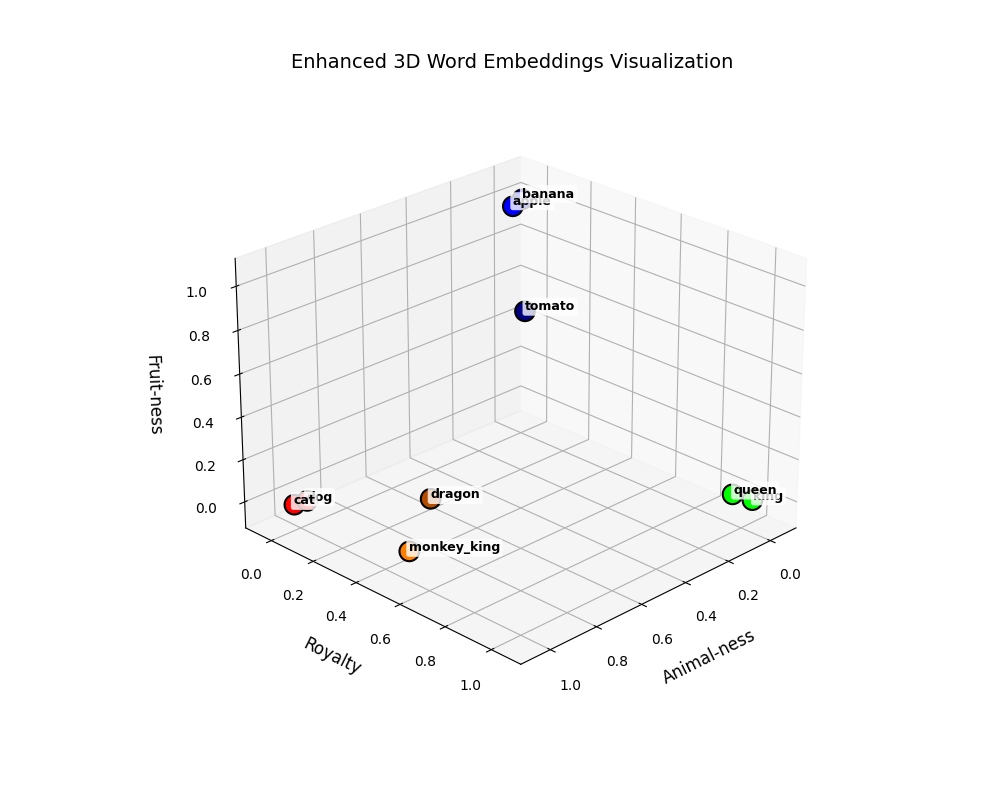
\includegraphics[width=8.4cm,height=4.8cm]{word_examples.png}
\par\end{center}
\small
The three axes loosely correspond to ``Animal-ness'', ``Royalty'', and ``Fruit-ness''. Words like \emph{cat}, \emph{king}, and \emph{apple} cluster along the dimension that fits them best. Real LLM embeddings live in hundreds of dimensions, but the same intuition holds.

{\footnotesize We compare words by the \emph{direction} of their vectors --- \textbf{cosine similarity} $\cos(\mathbf{u},\mathbf{v}) = \mathbf{u}^{\top}\mathbf{v} / (\|\mathbf{u}\|\|\mathbf{v}\|)$ --- not raw distance: frequent words grow longer vectors in training, and direction strips that out.}
\end{frame}

\begin{frame}{Analogies and the Bias Problem}
\begin{itemize}
\item \textbf{Geometric magic} (Mikolov et al., 2013): simple vector arithmetic captures analogies.
\[
   \mathbf{u}_{\text{king}} - \mathbf{u}_{\text{man}} + \mathbf{u}_{\text{woman}} \approx \mathbf{u}_{\text{queen}}
   \qquad
   \mathbf{u}_{\text{Paris}} - \mathbf{u}_{\text{France}} + \mathbf{u}_{\text{Italy}} \approx \mathbf{u}_{\text{Rome}}
\]

\medskip
\item Words on the same semantic axis differ by roughly the same vector --- gender, capital city, monetary stance. (Caveat: the clean pattern weakens for specialized, low-frequency vocabulary --- validate on your own terms.)

\medskip
\item \textbf{Bias is encoded too} (Bolukbasi et al., 2016, \emph{NeurIPS}; Caliskan, Bryson \& Narayanan, 2017, \emph{Science}):
\begin{itemize}
    \item $\mathbf{u}_{\text{man}} - \mathbf{u}_{\text{woman}}$ has a large component on \emph{programmer} vs.\ \emph{homemaker}.
    \item Word embeddings reproduce IAT-style biases at human magnitudes.
    \item For economic text: occupation/gender, race/credit-risk, region/sentiment correlations all transfer from the training corpus into the geometry.
\end{itemize}

\medskip
\item \textbf{Lesson:} embeddings are a mirror of the corpus. Checking that a sentiment vector tracks \emph{policy} stance and not \emph{speaker identity} is a real research step (returns in T5b) --- and the encoded bias can itself become the research object.
\end{itemize}
\end{frame}

\begin{frame}{Four Generations of Representation, One Table}
\textbf{Every step toward ``understanding'' trades away interpretability.}
\begin{center}
\renewcommand{\arraystretch}{1.35}
\small
\begin{tabular}{p{2.7cm} p{2.0cm} p{2.4cm} p{3.0cm}}
\toprule
 & \textbf{Counts / TF-IDF} & \textbf{Word2Vec} & \textbf{Contextual (BERT)} \\
\midrule
Captures meaning? & no (orthogonal) & yes (distributional) & strong (context-aware) \\
Same word, many senses? & no & one static vector & varies with context \\
Interpretable / auditable? & high (word $=$ axis) & low (latent space) & very low \\
Typical econ use & EPU, dictionaries & culture / network scores & sentiment, stance \\
\bottomrule
\end{tabular}
\end{center}
\medskip
\textbf{Rule:} when validity rests on an auditable, line-by-line evidence chain, the fancier representation is often the \emph{worse} choice. Pick the rung your research design needs --- not the newest one.
\end{frame}

\begin{frame}{From Analogies to Constructs: The Hawk--Dove Direction (Thread B)}
\textbf{Define an economic concept as a \emph{direction} in the space.}
\begin{itemize}
\item Candidate monetary-stance axis: $\hat{\mathbf{v}} = \mathbf{u}_{\text{hike}} - \mathbf{u}_{\text{cut}}$. Score any FOMC passage by the cosine of its (averaged) vector with $\hat{\mathbf{v}}$.
\item The same trick, generalized: culture scores from seed-word directions (Li, Mai, Shen \& Yan 2021); time-varying product-market networks from 10-K business-description similarity (Hoberg \& Phillips 2016).
\item \textbf{Validation idea:} a genuine stance direction should co-move with policy --- check the $\hat{\mathbf{v}}$-scores against subsequent fed-funds-rate changes before using them in a regression.
\end{itemize}
\medskip
\begin{cautionbox}
\textbf{The separability assumption.} \emph{king $-$ man $+$ woman} works because the difference is (mostly) one clean dimension --- everything else cancels. But \emph{hike} co-occurs with overheating and \emph{cut} with recessions, so $\hat{\mathbf{v}}$ may encode \textbf{stance and the business cycle at once} --- like a bond that bundles duration and credit risk in one price. Purge or control for the cycle dimension before calling it ``policy stance''; ask which institutional features make the coupling worse.
\end{cautionbox}
\end{frame}

\end{document}
